% Liu & Layland RMS utilization bound  U_lub(n) = n (2^{1/n} - 1)
% Compile:  pdflatex util_bound.tex  &&  dvisvgm --pdf util_bound.pdf
\documentclass[border=4pt]{standalone}
\usepackage{lmodern}
\usepackage{tikz}
\usetikzlibrary{arrows.meta}

\definecolor{kmblue}{HTML}{003874}
\definecolor{kmgold}{HTML}{BA9224}
\definecolor{rtgreen}{HTML}{1F9D55}
\definecolor{rtamber}{HTML}{D9A300}
\definecolor{rtred}{HTML}{E3342F}
\definecolor{dkgray}{HTML}{555555}

\begin{document}
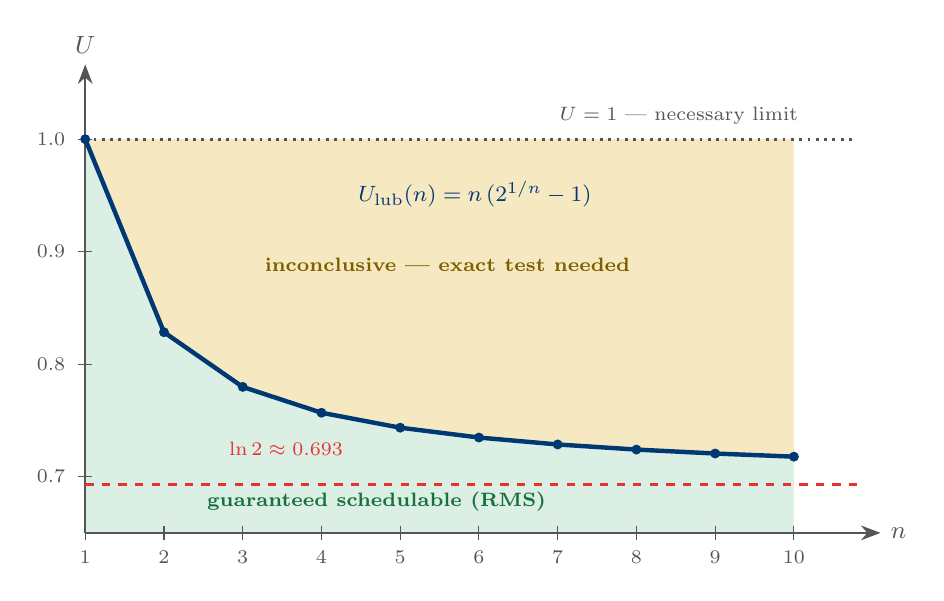
\begin{tikzpicture}[>=Stealth,font=\sffamily,x=1cm,y=1cm]

  % --- schedulable region (below the bound) ---
  \fill[rtgreen!16]
    (0,0) -- (0,5.000) -- (1,2.549) -- (2,1.854) -- (3,1.526)
    -- (4,1.336) -- (5,1.211) -- (6,1.123) -- (7,1.058)
    -- (8,1.008) -- (9,0.968) -- (9,0) -- cycle;
  % --- inconclusive region  (bound < U <= 1) ---
  \fill[rtamber!24]
    (0,5.000) -- (1,2.549) -- (2,1.854) -- (3,1.526)
    -- (4,1.336) -- (5,1.211) -- (6,1.123) -- (7,1.058)
    -- (8,1.008) -- (9,0.968) -- (9,5.000) -- cycle;

  % --- axes ---
  \draw[->,dkgray,line width=0.9pt] (0,0) -- (10.1,0)
        node[right,font=\small]{$n$};
  \draw[->,dkgray,line width=0.9pt] (0,0) -- (0,5.95)
        node[above,font=\small]{$U$};

  % y ticks
  \foreach \u/\yy in {0.7/0.714,0.8/2.143,0.9/3.571,1.0/5.000} {
    \draw[dkgray] (-0.09,\yy) -- (0.09,\yy);
    \node[dkgray,font=\scriptsize,left] at (-0.13,\yy) {\u};
  }
  % x ticks
  \foreach \n/\xx in {1/0,2/1,3/2,4/3,5/4,6/5,7/6,8/7,9/8,10/9} {
    \draw[dkgray] (\xx,-0.09) -- (\xx,0.09);
    \node[dkgray,font=\scriptsize,below] at (\xx,-0.11) {\n};
  }

  % U = 1 reference line
  \draw[dkgray,dotted,line width=1.0pt] (0,5.000) -- (9.8,5.000);
  \node[dkgray,font=\scriptsize,right] at (5.9,5.30)
        {$U=1$ --- necessary limit};

  % ln 2 asymptote
  \draw[rtred,dashed,line width=1.0pt] (0,0.616) -- (9.8,0.616);
  \node[rtred,font=\scriptsize] at (2.55,1.07)
        {$\ln 2 \approx 0.693$};

  % the bound curve
  \draw[kmblue,line width=1.6pt]
    (0,5.000) -- (1,2.549) -- (2,1.854) -- (3,1.526)
    -- (4,1.336) -- (5,1.211) -- (6,1.123) -- (7,1.058)
    -- (8,1.008) -- (9,0.968);
  \foreach \p in {(0,5.000),(1,2.549),(2,1.854),(3,1.526),(4,1.336),
                  (5,1.211),(6,1.123),(7,1.058),(8,1.008),(9,0.968)}
    \fill[kmblue] \p circle (1.8pt);

  % labels
  \node[kmblue,font=\footnotesize\bfseries] at (4.95,4.30)
        {$U_{\mathrm{lub}}(n)=n\,(2^{1/n}-1)$};
  \node[rtamber!58!black,font=\scriptsize\bfseries] at (4.6,3.40)
        {inconclusive --- exact test needed};
  \node[rtgreen!72!black,font=\scriptsize\bfseries] at (3.7,0.40)
        {guaranteed schedulable (RMS)};

\end{tikzpicture}
\end{document}
